\section{Introduction}

Heterogeneous information networks (HINs) model real-world systems with multiple node and edge types, such as bibliographic networks (authors, papers, venues), e-commerce platforms (users, products, categories), and knowledge graphs (entities, relations, types). Community search---finding a cohesive subgraph containing a given query node---is a fundamental operation over HINs, with applications in expert recommendation, fraud ring detection, and product suggestion~\cite{zhang2025scsh,sach2024icde}.

Zhang et al.~\cite{zhang2025scsh} recently formalized the \emph{size-constrained} community search problem over HINs (SCSH), which seeks a community of exactly $s$ nodes maximizing the $(k,\mathcal{P})$-truss cohesiveness metric. They proved the problem NP-hard and proposed exact Branch \& Bound algorithms with polynomial-time heuristics. However, their solution is fundamentally \emph{static}: any change to the graph requires recomputing the community from scratch.

This static assumption is at odds with reality. HINs evolve continuously: authors publish new papers, customers purchase additional products, and entities acquire new relationships. Recomputing communities from scratch after each update incurs substantial latency---in our reported synthetic and hybrid runs, the fixed-query greedy baseline averages roughly 390--950~ms per checkpointed recomputation. For applications such as interactive expert recommendation or fraud monitoring where updates arrive at sub-second intervals, this per-update cost cannot be amortized: the recomputation latency exceeds the inter-update gap, making static recomputation a throughput bottleneck even at modest graph scales.

The natural question is: \emph{Can we maintain size-constrained communities incrementally as the graph evolves, avoiding the cost of full recomputation?}

This paper answers affirmatively with \textbf{\DynaSCSH}, the first dynamic size-constrained community search framework for evolving HINs. \DynaSCSH combines three novel components:

\begin{enumerate}
\item \textbf{Meta-Path Triangle Index (\mtindex):} A count-based $O(|E|)$ index tracking meta-path triangle participation per edge, updated in $O(d_{\mathcal{P}}(u)\cdot d_{\mathcal{P}}(v))$ time per edge change. Triangle structures are resolved on-demand during cascading truss collapse rather than pre-materialized, avoiding the $O(|E|\cdot d_{\max}^2)$ memory explosion of explicit triangle storage.

\item \textbf{Internal Support Cache:} A running dictionary of $(k,\mathcal{P})$-truss support counts for edges \emph{within} the maintained community, computed strictly over the induced subgraph. This makes validation independent of the full graph size and exposes the common fast path where a projected-edge update does not touch the maintained community.

\item \textbf{Localized Repair with Validated Fallback:} When community edges are deleted, \DynaSCSH searches for replacement nodes within a bounded hop radius. A repaired community is returned only after checking size, original query containment, internal support, and triangle connectivity. If no candidate passes validation, \DynaSCSH falls back to the same fixed-query greedy recomputation used by the static baseline.
\end{enumerate}

We evaluate \DynaSCSH in two evidence-backed settings: 22 fixed-query synthetic DBLP configurations and a separate 26,850-node hybrid benchmark combining real DBLP topology with planted dense communities.

\textbf{Key findings (post-fix, fixed-query baseline, 22 configurations):}
\begin{itemize}
\item \textbf{Insertion streams:} With a fixed query node, \DynaSCSH preserves structure exactly (Jaccard=1.000 in all 17 insertion runs) and keeps quality at parity on average (\qratio=1.000), with 3,824$\times$ average speedup.
\item \textbf{Deletion streams:} Deletions diverge naturally: Jaccard 0.36--0.54 and \qratio 0.89--0.92. They still average 2,188$\times$ speedup; D1 drops to 1.4$\times$ when fallback dominates.
\item \textbf{Invariant-checked repair:} Local repair is accepted only after support, size, query containment, and triangle connectivity checks; otherwise the framework falls back to fixed-query greedy recomputation.
\item \textbf{Planted Community Benchmark:} On a 26,850-node hybrid graph (real DBLP topology + 40 planted dense communities), \DynaSCSH achieves 5,900--10,700$\times$ speedup under the fixed-query baseline, preserves community identity (Jaccard=1.000 across the reported hybrid insertion/deletion streams), and repairs 10/30 targeted community-edge deletions at $k$=2.
\end{itemize}

\begin{figure*}[htbp]
\centering
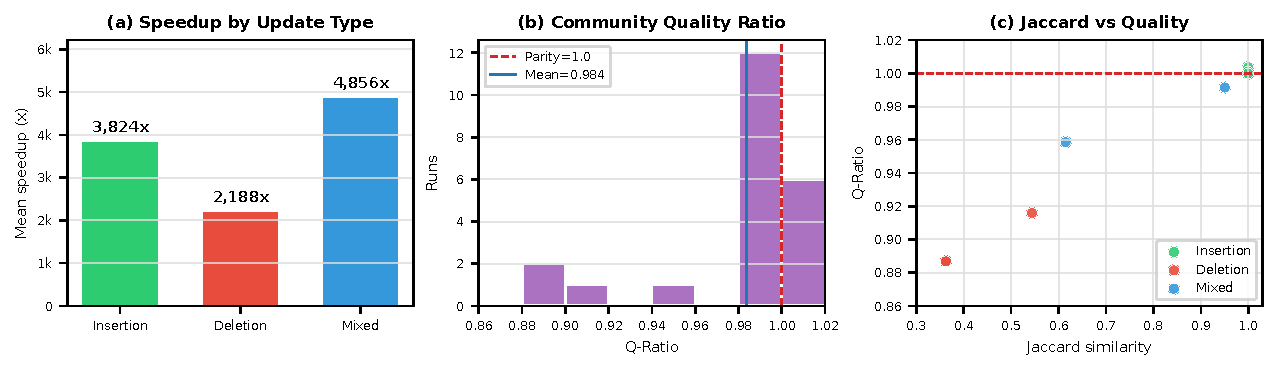
\includegraphics[width=.78\textwidth]{figures/fig_teaser.pdf}
\caption{Overview under the fixed-query baseline. (a) Speedups by update type on the synthetic benchmark. (b) \qratio distribution across 22 configurations. (c) Jaccard vs.\ \qratio, showing that structural overlap and score can diverge even when dynamic and static methods use the same query.}
\Description{Three-panel teaser showing speedups, quality-ratio distribution, and Jaccard versus Q-Ratio under the fixed-query baseline.}
\label{fig:teaser}
\end{figure*}
